\documentclass[12pt]{article}
\usepackage{graphicx}
\usepackage{wrapfig}
\usepackage{amsmath}
\usepackage[brazil]{babel}
\usepackage[a4paper, left=3cm, top=3cm, right=2cm, bottom=2cm]{geometry}
\usepackage{float}
\usepackage{hyperref}
\usepackage[square,numbers]{natbib}
\setcounter{secnumdepth}{4}
\setcounter{tocdepth}{4}
\bibliographystyle{abbrvnat}

\setcounter{secnumdepth}{4}  % Permite numerar até nível 4
\setcounter{tocdepth}{4}     % Inclui nível 4 no sumário

\newcommand{\subsubsubsection}[1]{%
  \paragraph{#1}\mbox{}\\
}

\begin{document}


\begin{titlepage}
    \begin{center}
        Universidade Federal de Santa Catarina\\
        Departamento de Engenharias da Mobilidade \\ Eletrônica Análogica - EMB5116\\

        \vspace{1.5cm}
        
\includegraphics[width=0.28\textwidth]{./images/vertical_sigla_fundo_claro.png}

        \vspace*{1.5cm}
        \fontsize{12pt}{16pt}\textbf{Eletrônica Analógica - Trabalho 2}

        \vspace*{1.5cm}
        Dr. Prof. Milton Evangelista de Oliveira Filhos

        \vspace*{1.0cm}
        \begin{tabular}{c c}
                André Stein - 22201053\\
                Danilo Machado - 22203056\\
                Pedro Lauxen - 22201064\\
        \end{tabular}

        \vspace*{\fill}
        {Joinville\\
        2025}
    \end{center}
\end{titlepage}


\tableofcontents\renewcommand*\contentsname{Sumário}
\newpage

\section{Introdução}

    Dispositivos transistores são utilizados comumente como meios de amplificar, ou chavear um circuito, de forma que o mesmo opere da maneira desejada no circuito. Dentre os transistores existentes os tipos mais comuns são os bipolares de junção,cujo são componentes formados pela junção de semicondutores,de forma que os agregando em conjuntos do tipo NPN ou PNP, forma-se um dispositivo que opera conforme é configurada sua polarização, porém assim como há a existência de componentes específicos dentro do mundo dos capacitores e resistores, dentro do mundo dos transistores existem os transistores de efeito de campo, que utilizam outra forma de controlar o fluxo de corrente por semicondutores. Neste trabalho serão descritos diferentes transistores de efeito de campo(FET) como,FET de junção (JFET),FET de Metal-Óxido-Semicondutor(MOSFET) e por último o Transistor Bipolar de Porta Isolada(IGBT) determinando como funciona cada um desses componentes, assim como será feita a comparação entre os mesmos, e por fim a comparação direta com transistores bipolares de junção.

\newpage


\section{FET de junção(JFET)}

O transistor de efeito de campo de junção, conhecido com JFET, é um dos dispositivos semicondutores mais importantes na eletrônica analógica. Ele opera a partir do controle do fluxo de portadores de carga em um canal semicondutor através de um campo elétrico aplicado a uma junção PN. Ao contrário do transistor bipolar (BJT), o JFET é controlado por tensão, o que confere ao dispositivo alta impedância de entrada e baixo consumo de energia, assim o JFET não carrega o circuito anterior, sendo ideal como estágio de entrada em amplificadores.

        \begin{figure}[htpb!]
            \centering
            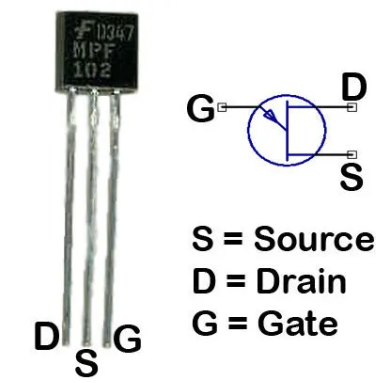
\includegraphics[width=0.3\linewidth]{images/Captura de tela 2025-10-18 223003.png}
            \caption{Transistor JFET}
        \end{figure}

\subsection{Histórico do Transistor JFET}

 Sua concepção teórica foi inicialmente proposta em 1928 por Julius Edgar Lilienfeld, que descreveu o princípio de controle de corrente por meio de um campo elétrico aplicado a um semicondutor. No entanto, na época, as limitações tecnológicas relacionadas à pureza dos materiais semicondutores e à ausência de técnicas avançadas de fabricação impediram a implementação prática do dispositivo.

Somente a partir da década de 1950, com o avanço dos processos de dopagem e crescimento controlado de cristais de silício e germânio, tornou-se possível fabricar JFETs funcionais. Empresas como a Bell Labs e a Fairchild Semiconductor tiveram papel fundamental no aperfeiçoamento da tecnologia. O JFET tornou-se, o primeiro tipo de transistor de efeito de campo fabricado, antecedendo os MOSFETs.


\subsection{Princípio de Funcionamento}


O JFET é um dispositivo semicondutor de três terminais: Gate (G), Source (S) e Drain (D). Seu funcionamento baseia-se no controle do fluxo de portadores de carga através de um canal semicondutor (de tipo N ou P), que é modulado pela tensão aplicada entre o gate e a fonte.

\begin{itemize}
    \item \textbf{Gate (G) — Porta:} É o terminal responsável pelo controle do fluxo de corrente no canal.
    O gate é formado por uma junção PN polarizada reversamente em relação ao canal, o que faz com que praticamente não haja corrente fluindo pelo gate.
    A tensão aplicada entre o gate e a fonte ($V_{GS}$) cria um campo elétrico que modula a largura efetiva do canal, controlando assim a corrente que circula entre o dreno e a fonte.

    \item \textbf{Source (S) — Fonte:} É o terminal por onde os portadores de carga entram no canal.
    Para um JFET de canal N, os portadores são elétrons; para um JFET de canal P, são lacunas.
    A tensão do gate é sempre medida em relação à fonte ($V_{GS}$), tornando o \textit{source} o terminal de referência para o controle do dispositivo.

    \item \textbf{Drain (D) — Dreno:} É o terminal por onde os portadores de carga saem do canal após percorrê-lo.
    A corrente que flui do dreno para a fonte ($I_D$) depende da tensão $V_{GS}$ aplicada ao gate e da tensão $V_{DS}$ aplicada entre o dreno e a fonte.
    Quando $V_{GS}$ se torna mais negativo (no caso de um JFET de canal N), a região de depleção se expande, estreitando o canal e reduzindo a corrente $I_D$, até o ponto de corte (pinch-off).
\end{itemize}

        \begin{figure}[htpb!]
            \centering
            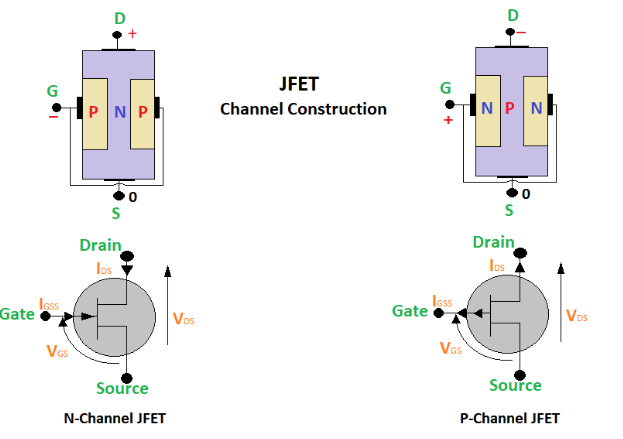
\includegraphics[width=0.8\linewidth]{images/pn.png}
            \caption{Representação de um JFET}
        \end{figure}

\subsubsection{Fluxo de Corrente no Canal}

Quando uma tensão \(V_{DS}\) é aplicada entre o dreno e a fonte, uma corrente \(I_D\) começa a fluir através do canal, composta por elétrons (no JFET de canal N) ou lacunas (no JFET de canal P). A magnitude dessa corrente depende da largura efetiva do canal condutor.

O gate é uma junção PN polarizada reversamente. Isso significa que praticamente não há corrente de gate, pois a barreira de potencial impede o fluxo de portadores. Entretanto, a região de depleção da junção se expande, reduzindo a seção transversal do canal e, consequentemente, controlando a corrente \(I_D\).


        \begin{figure}[htpb!]
            \centering
            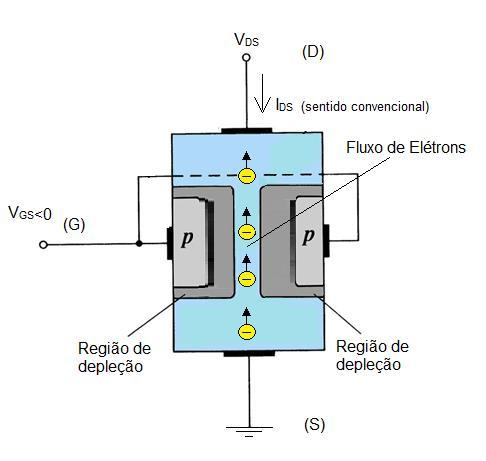
\includegraphics[width=0.5\linewidth]{images/JFET-de-canal-n-reversamente-polarizado-corpo-com-cargas-negativas-nas-proximidades-da.png}
            \caption{JFET de canal n reversamente polarizado}
            \label{fig:JFET}
        \end{figure}

\subsubsection{Efeito da Polarização do Gate}

O gate é constituído por uma junção PN polarizada reversamente em relação ao canal. Nessa condição, praticamente não há corrente fluindo pelo gate, pois a barreira de potencial da junção impede o movimento de portadores de carga. Apesar disso, a polarização reversa provoca o alargamento da região de depleção, que se estende lateralmente a partir das junções PN em direção ao interior do canal.

À medida que a tensão $V_{GS}$ (tensão entre gate e source) se torna mais negativa no caso de um JFET de canal N, a região de depleção se expande, reduzindo a largura efetiva do canal condutor. Com a diminuição dessa seção transversal, a resistência do canal aumenta, resultando em uma diminuição da corrente $I_D$. Esse mecanismo de controle é o que caracteriza o funcionamento do JFET como um dispositivo de efeito de campo, o campo elétrico gerado pela tensão no gate modula a condutância do canal.

        \begin{figure}[htpb!]
            \centering
            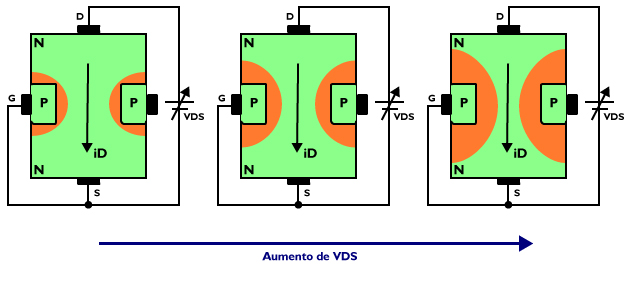
\includegraphics[width=0.8\linewidth]{images/aumento Vds.png}
            \caption{Representação da região de depleção}
        \end{figure}

\subsubsection{Equação de Shockley}

A característica fundamental do JFET é o controle da corrente do canal por meio do campo elétrico estabelecido pela tensão \(V_{GS}\).
Para um JFET de canal N:
\begin{itemize}
    \item Quando \(V_{GS} = 0\), o canal apresenta sua máxima condutividade, e a corrente \(I_D\) atinge o valor máximo \(I_{DSS}\).

    \item À medida que \(V_{GS}\) torna-se negativo, as regiões de depleção em torno do gate aumentam, estreitando o canal e reduzindo \(I_D\).

    \item Quando \(V_{GS}\) atinge a tensão de corte \(V_P\), o canal é completamente bloqueado, e \(I_D \approx 0\).
\end{itemize}

Esse comportamento é representado pela Equação de Shockley:
\[
I_D = I_{DSS} \left( 1 - \frac{V_{GS}}{V_P} \right)^2
\]

\subsubsection{Regiões de Operação}

Para o transistor JFET pode-se distinguir três regiões principais de operação:

\begin{enumerate}
    \item \textbf{Região ôhmica (ou linear):}
    Quando $V_{DS}$ é pequeno, a corrente $I_D$ é aproximadamente proporcional à tensão $V_{DS}$, obedecendo uma relação quase linear. O dispositivo atua como um resistor controlado por tensão, e o canal permanece totalmente aberto.

    \item \textbf{Região de saturação (ou ativa):}
    À medida que $V_{DS}$ aumenta, a tensão no dreno se torna mais positiva em relação ao gate, fazendo com que a região de depleção se expanda mais próxima ao dreno do que ao source.
    Em um ponto específico, conhecido como tensão de estrangulamento ou pinch-off ($V_P$), as regiões de depleção provenientes das laterais do canal se encontram, estrangulando-o.
    A partir desse ponto, o aumento de $V_{DS}$ não causa um aumento significativo em $I_D$, e a corrente se torna praticamente constante.
    O JFET opera, então, como uma fonte de corrente controlada por tensão.

    \item \textbf{Região de corte:}
    Quando $V_{GS}$ é suficientemente negativo (em módulo igual ou superior a $V_P$), o canal é completamente bloqueado pela expansão das regiões de depleção, impedindo o fluxo de corrente. Nessa condição, $I_D$ é aproximadamnete 0.
\end{enumerate}

        \begin{figure}[htpb!]
            \centering
            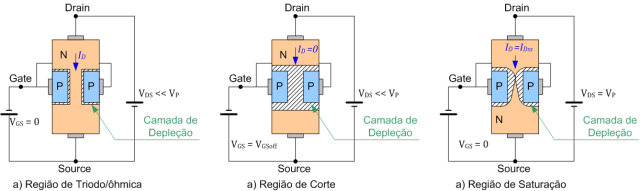
\includegraphics[width=1.0\linewidth]{images/regioes.png}
            \caption{Representação de cada região}
        \end{figure}


\subsection{Construção e Design do JFET}

\subsubsection{Estrutura Física}

O JFET é construído a partir de um cristal semicondutor (geralmente silício) no qual se define um canal condutor de tipo N ou tipo P. O canal é cercado por regiões de dopagem oposta, que formam junções PN com o canal, conhecidas como regiões de gate. Como pode ser notado na  figura \ref{fig:JFET}.

Características da estrutura física:

\begin{itemize}
    \item \textbf{Canal semicondutor:} É levemente dopado para permitir controle eficaz da corrente, mantendo o valor de \(I_{DSS}\) dentro das especificações. O canal é formado longitudinalmente entre os terminais source e drain.


    \item \textbf{Junções Gate-Canal:} As regiões de dopagem do gate são fortemente dopadas para formar junções PN eficientes. A polarização reversa dessas junções controla a largura efetiva do canal.

    \item \textbf{Terminais Source e Drain:} Conectados nas extremidades do canal, permitem a entrada e saída de portadores de carga.

    \item \textbf{Substrato:} Pode estar conectado ao gate (common gate) ou flutuante, dependendo do design. Em alguns casos, o substrato é de tipo oposto ao canal e atua como um dissipador térmico e suporte mecânico.
\end{itemize}

\subsubsection{Considerações de Dopagem e Materiais}

O controle da dopagem é crítico no projeto de JFETs, pois determina parâmetros elétricos essenciais:

\begin{itemize}
    \item Dopagem do canal: Uma dopagem mais leve aumenta a resistência do canal e permite maior controle da corrente pelo gate, mas reduz \(I_{DSS}\).

    \item Dopagem do gate: Alta dopagem assegura junções PN de baixa resistência e pequena capacitância reversa, fundamental para alta frequência.

    \item Material semicondutor: Silício é predominante, mas arseneto de gálio (GaAs) é usado em JFETs de RF devido à maior mobilidade de elétrons e menor ruído.
\end{itemize}

\subsubsection{Geometria do Canal}

A geometria do canal é um dos fatores mais críticos no projeto de um JFET, influenciando diretamente o comportamento elétrico, térmico e a linearidade do dispositivo. O canal é caracterizado principalmente pelo seu comprimento \(L\), largura \(W\) e espessura \(t\), além do perfil de dopagem.

A geometria do canal determina diretamente os parâmetros elétricos fundamentais, como \(I_{DSS}\), \(V_P\), \(g_m\), linearidade, resposta em frequência e dissipação térmica. O projeto exige um equilíbrio cuidadoso entre largura, comprimento, espessura e dopagem para atender às especificações do circuito.

\subsubsubsection{Comprimento do Canal (\(L\))}

O comprimento do canal, medido entre os terminais source e drain impactam:

\begin{itemize}
    \item \textbf{Resistência do canal:} Um canal mais longo aumenta a resistência ôhmica \(R_{DS(on)}\), reduzindo a corrente máxima \(I_{DSS}\). A relação aproximada é \((R \propto L)/W\), considerando dopagem uniforme.

    \item \textbf{Linearidade em pequenos sinais:} Canais longos distribuem melhor o campo elétrico, reduzindo a distorção harmônica em amplificadores de baixa tensão.

    \item \textbf{Controle do pinch-off:} Comprimentos maiores tornam a transição entre a região ôhmica e a saturação mais suave, melhorando o controle da corrente.

    \item \textbf{Efeito de capacitâncias parasitas:} Canais longos podem aumentar a capacitância gate-drain \(C_{GD}\), afetando a resposta em alta frequência.
\end{itemize}

\subsubsubsection{Largura do Canal (\(W\))}

A largura do canal afeta:

\begin{itemize}
    \item \textbf{Corrente máxima:} Quanto maior a largura, maior a área condutora disponível, portanto maior \(I_{DSS}\).
    \item \textbf{Distribuição da densidade de corrente:} Canais muito estreitos podem concentrar a densidade de corrente, gerando aquecimento localizado e instabilidade térmica.
    \item \textbf{Sensibilidade à tensão do gate:} Larguras menores tornam o dispositivo mais sensível a variações de \(V_{GS}\), pois a região de depleção ocupa uma fração maior do canal.
\end{itemize}

\subsubsubsection{Espessura e Perfil de Dopagem do Canal}

A espessura efetiva do canal e o perfil de dopagem influenciam:

\begin{itemize}
    \item \textbf{Resistência de condução:} Canais mais finos ou menos dopados aumentam a resistência e reduzem \(I_{DSS}\), mas melhoram a linearidade.

    \item \textbf{Uniformidade do campo elétrico:} Perfis de dopagem gradientes permitem uma variação controlada da resistência ao longo do canal, suavizando o efeito de pinch-off.

    \item \textbf{Ruído térmico:} Canais finos geram menos corrente de ruído, essencial em aplicações de instrumentação de precisão.
\end{itemize}

\subsubsubsection{Relação Largura/Comprimento (\(W/L\))}

A razão \(W/L\) é frequentemente usada como parâmetro de projeto:

\begin{itemize}
    \item \textbf{Alta \(W/L\):} Favorece alta corrente \(I_{DSS}\) e menor resistência do canal, mas pode aumentar capacitâncias parasitas e reduzir linearidade.

    \item \textbf{Baixa \(W/L\):} Melhora linearidade e controle de corrente, mas limita \(I_{DSS}\) e aumenta a resistência.
\end{itemize}

Essas técnicas tornam os JFETs adequados para instrumentação, áudio de alta fidelidade e circuitos analógicos de precisão.

\subsection{Aplicações dos Transistores JFET}

\subsubsection{Amplificadores de Baixo Ruído}

Devido à sua alta impedância de entrada e baixo ruído térmico, os JFETs são amplamente usados em:

\begin{itemize}
    \item \textbf{Pré-amplificadores de microfone:} Mantêm a integridade do sinal e minimizam a interferência de ruído da fonte de sinal.

    \item \textbf{Amplificadores de instrumentação:} Em sistemas de medição de sinais muito pequenos, como sensores de temperatura ou tensão de strain gauge.

    \item \textbf{Amplificadores de áudio de alta fidelidade:} Garantem mínima distorção e preservação do espectro sonoro.
\end{itemize}

\subsubsection{Circuitos de Entrada de Instrumentação}

A elevada impedância de entrada torna o JFET ideal para circuitos onde a carga do sinal deve ser mínima:

\begin{itemize}
    \item \textbf{Osciloscópios e voltímetros de alta impedância:} Evitam carregamento do circuito sob teste.

    \item \textbf{Buffers (source followers):} Isolam estágios sensíveis, mantendo a amplitude e forma do sinal.

    \item \textbf{Amplificadores diferenciais de precisão:} Reduzem o erro devido a correntes de polarização.
\end{itemize}

\subsubsection{Fontes de Corrente Constante e Circuitos de Controle}

O JFET, em região de saturação, atua como uma fonte de corrente controlada por tensão:

\begin{itemize}
    \item \textbf{Fontes de corrente constantes:} Usadas em circuitos de polarização de transistores bipolares ou MOSFETs, proporcionando estabilidade térmica.

    \item \textbf{Circuitos de referência de corrente:} Mantêm corrente estável independentemente da tensão de alimentação.

    \item \textbf{Cascodes e espelhos de corrente:} Melhoram a faixa de ganho e a linearidade.
\end{itemize}

\subsubsection{Chaves Eletrônicas e Comutação Analógica}

JFETs são excelentes para chaves analógicas devido à baixa resistência de canal em região ôhmica:

\begin{itemize}
    \item \textbf{Multiplexadores analógicos:} Selecionam sinais sem degradar a amplitude ou forma de onda.

    \item \textbf{Chaves de áudio de alta fidelidade:} Evitam distorção em equipamentos de som profissional.

    \item \textbf{Amostragem de sinais:} Aplicações em conversores A/D e circuitos de medição.
\end{itemize}

\subsubsection{Circuitos de Alta Frequência e RF}

Apesar de não serem tão rápidos quanto MOSFETs de efeito de campo de óxido, JFETs são usados em RF devido à baixa capacitância de entrada:

\begin{itemize}
    \item \textbf{Osciladores de RF:} Estabilidade de frequência e baixo ruído.

    \item \textbf{Amplificadores de RF de baixo nível:} Como primeiros estágios em receptores de rádio e TV.

    \item \textbf{Misturadores e moduladores:} Precisão em circuitos de comunicação analógica.
\end{itemize}

\subsubsection{Aplicações em Sensores e Circuitos de Precisão}

O JFET é ideal em sensores devido à sua estabilidade e baixa corrente de fuga:

\begin{itemize}
    \item \textbf{Sensores de capacitância ou piezoelétricos:} O JFET não descarrega o sinal detectado.

    \item \textbf{Medidores de carga ou fotodiodos:} Minimiza corrente de polarização de entrada.

    \item \textbf{Amplificadores de instrumentação médica:} Eletrocardiogramas (ECG) e eletroencefalogramas (EEG).
\end{itemize}

\subsubsection{Outras Aplicações Especiais}

\begin{itemize}
    \item \textbf{Circuitos de proteção:} Limitadores de corrente em linhas sensíveis.
    \item \textbf{Modulação de sinais:} Em moduladores analógicos de amplitude ou frequência.
    \item \textbf{Pré-amplificadores de imagem e vídeo:} Onde baixa corrente de entrada e alta linearidade são essenciais.
    \item \textbf{Amplificadores operacionais JFET:} Amplificadores integrados com alto ganho e baixa corrente de bias.
\end{itemize}


\subsection{Comparação entre JFET e Transistor Bipolar (BJT)}

A seguir, são apresentadas as principais diferenças entre o JFET e o BJT, destacando aspectos de controle, impedância, ruído, estabilidade e faixa de frequência.

\begin{itemize}
    \item \textbf{Tipo de Controle:}
    \begin{itemize}
        \item JFET: Controlado por tensão (\(V_{GS}\)), resultando em menor consumo de energia e mínima corrente de entrada.
        \item BJT: Controlado por corrente (\(I_B\)), exigindo corrente de base para operar.
    \end{itemize}

    \item \textbf{Impedância de Entrada:}
    \begin{itemize}
        \item JFET: Impedância de entrada muito alta, da ordem de megaohms ou superior, evitando carregamento do circuito anterior.
        \item BJT: Impedância de entrada relativamente baixa, limitada pela base, o que pode afetar estágios sensíveis de sinal.
    \end{itemize}

    \item \textbf{Ruído e Estabilidade:}
    \begin{itemize}
        \item JFET: Apresenta menor ruído de entrada e maior estabilidade térmica, ideal para instrumentação e aplicações de precisão.
        \item BJT: Maior ganho de corrente, mas sensível à variação térmica; preferido em estágios de potência e amplificação de sinais maiores.
    \end{itemize}

    \item \textbf{Faixa de Frequência:}
    \begin{itemize}
        \item JFET: Pode operar em frequências elevadas, adequado para circuitos de RF de baixo nível.
        \item BJT: Mais eficiente em altas potências de RF, devido à maior mobilidade de portadores e capacidade de conduzir correntes mais elevadas.
    \end{itemize}
\end{itemize}


\section{FET de Metal-Óxido-Semicondutor(MOSFET)}

        \begin{figure}[htpb!]

            \centering
            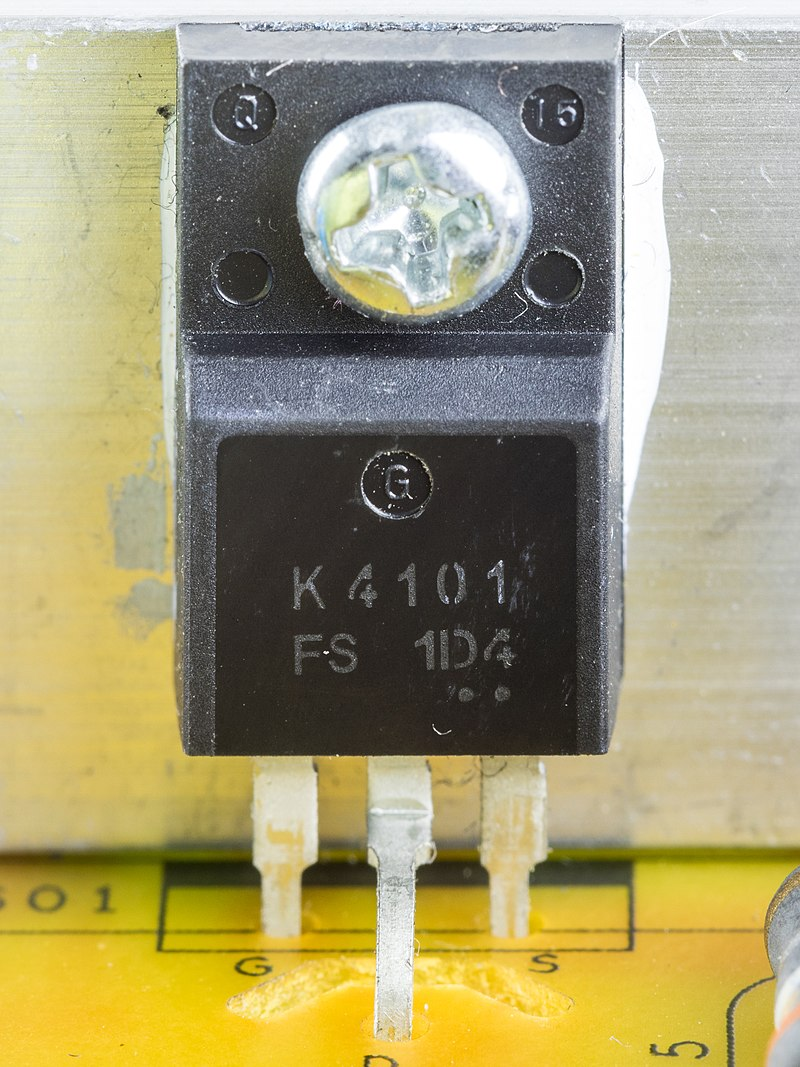
\includegraphics[width=0.2\textwidth]{./images/Dell_Professional_P2212H_-_power_supply_board_-_K4101FS-2149.jpg}
            \caption{MOSFET de potência.}

        \end{figure}

    O transistor MOSFET (acrônimo de Metal Oxide Semiconductor Field Effect Transistor, ou transistor de efeito de campo semicondutor de óxido metálico — TECMOS), é o tipo mais comum de transístores de efeito de campo em circuitos tanto digitais quanto analógicos. Seu princípio básico foi proposto pela primeira vez por Julius Edgar Lilienfeld, em 1925.
\cite{wikipedia_mosfet_2025}

    Os transistores de efeito de campo diferentemente dos transistores bipolares comuns são típicos amplificadores de tensão e não de corrente. Enquanto a corrente de coletor de um transistor comum é função da corrente de base, num transistor de efeito de campo, a corrente de dreno é função da tensão de comporta, conforme indica a figura \ref{fig:comparacao}.

        \begin{figure}[htpb!]

            \centering
            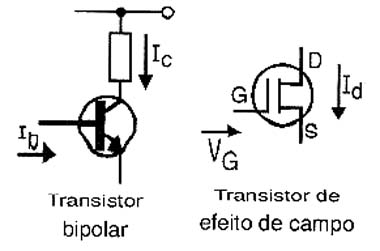
\includegraphics[width=0.4\textwidth]{./images/transisCampo.jpg}
            \caption{comparação entre transistor bipolar e transistor de efeito de campo.}
            \label{fig:comparacao}

        \end{figure}

        \begin{figure}[htpb!]

            \centering
            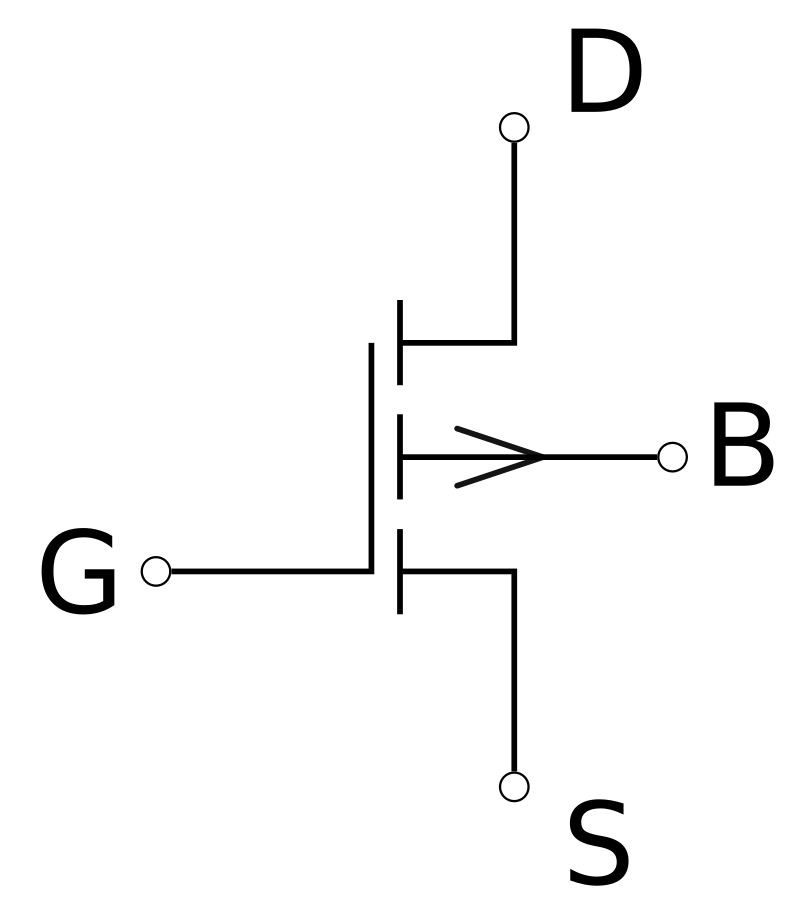
\includegraphics[width=0.2\textwidth]{./images/Mosfet-wp.svg.png}
            \caption{Símbolo de esquema elétrico de um MOSFET.}

        \end{figure}

    Uma fina película de óxido de metal isola a região de comporta da região do canal que liga o dreno à fonte. Isso faz com que a impedância de entrada do MOSFET seja muito alta, o que significa que ele consome muito pouca corrente da fonte de sinal que está dirigindo a comporta. Essa característica torna os MOSFETs ideais para circuitos de alta impedância, como amplificadores de áudio e circuitos digitais. Além disso, os MOSFETs são capazes de operar em frequências muito altas, tornando-os adequados para aplicações em rádio frequência (RF) e micro-ondas.

        \begin{figure}[htpb!]

            \centering
            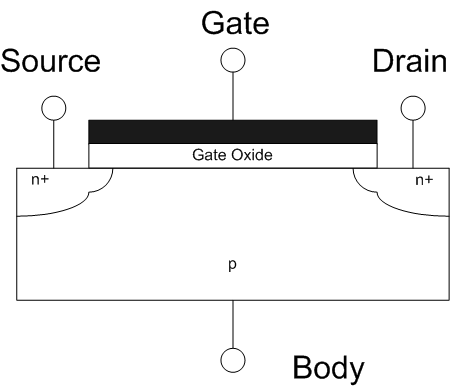
\includegraphics[width=0.3\textwidth]{./images/FET_cross_section.png}
            \caption{Símbolo de esquema elétrico de um MOSFET.}

        \end{figure}

    A palavra "metal" no nome é um anacronismo vindo dos primeiros chips, onde as comportas (gates) eram de metal. Os chips modernos usam comportas de polissilício, mas ainda são chamados de MOSFETs. Um MOSFET é composto de um canal de material semicondutor de tipo N ou de tipo P e é chamado respectivamente de NMOS ou PMOS. Geralmente o semicondutor escolhido é o silício, mas alguns fabricantes, principalmente a IBM, começaram a usar uma mistura de silício e germânio (SiGe) nos canais dos MOSFETs. Infelizmente muitos semicondutores com melhores propriedades elétricas do que o silício, tais como o arsenieto de gálio, não formam bons óxidos nas comportas e portanto não são adequados para os MOSFETs. O IGFET é um termo relacionado que significa Insulated-Gate Field Effect Transistor, e é quase sinônimo de MOSFET, embora ele possa se referir a um FET com comporta isolada por um isolante não óxido.

    O terminal de comporta é uma camada de polissilício (sílicio policristalino) colocada sobre o canal, mas separada do canal por uma fina camada de dióxido de silício isolante. Quando uma tensão é aplicada entre os terminais comporta (gate) e fonte (source), o campo elétrico gerado penetra através do óxido e cria uma espécie de "canal invertido" no canal original abaixo dele. O canal invertido é do mesmo tipo P ou tipo N, como o da fonte ou do dreno, assim, ele cria um condutor através do qual a corrente elétrica possa passar. Variando-se a tensão entre a comporta e a fonte se modula a condutividade dessa camada e torna possível se controlar o fluxo de corrente entre o dreno e a fonte. Existem também modelos de Amplificador operacional baseados na tecnologia FET/MOSFET, muito úteis e com grande utilização na indústria eletrônica.

        \subsection{Estrutura do MOSFET}

            O MOSFET é um dispositivo de quatro terminais: dreno (drain), fonte (source), porta (gate) e substrato (bulk). Em dispositivos discretos o substrato costuma estar ligado à fonte, de modo que apenas três terminais são acessíveis. Dois parâmetros geométricos importantes são a largura do canal $W$ e o comprimento do canal $L$. A espessura da camada de óxido da porta, $t_{ox}$, determina a capacitância por unidade de área $C_{ox}$; em geral, quanto menor $t_{ox}$, maior $C_{ox}$ e maior a influência da tensão de porta sobre o canal.

        \subsection{Modos de operação do MOSFET}

            A operação do MOSFET (assumindo NMOS) pode ser dividida em três regimes principais:

                \begin{itemize}

                    \item \textbf{Região de corte:} quando $V_{GS}<V_{th}$. O canal não está formado e o transistor permanece desligado (apenas corrente de fuga).

                    \item \textbf{Região linear (triode):} quando $V_{GS}>V_{th}$ e $V_{DS}<V_{GS}-V_{th}$. Nesta região o canal está formado por toda a extensão entre dreno e fonte e o MOSFET se comporta aproximadamente como um resistor controlado por $V_{GS}$. Uma expressão aproximada da corrente de dreno é
                    \[
                    I_D = \mu_n C_{ox} \frac{W}{L}\left((V_{GS}-V_{th})V_{DS}-\tfrac{1}{2}V_{DS}^2\right),
                    \]
                    onde $\mu_n$ é a mobilidade dos portadores e $C_{ox}$ a capacitância do óxido por unidade de área.

                    \item \textbf{Região de saturação:} quando $V_{GS}>V_{th}$ e $V_{DS}\ge V_{GS}-V_{th}$. O canal sofre "pinch-off" próximo ao dreno e a corrente de dreno aproxima-se de
                    \[
                    I_D = \tfrac{1}{2}\,\mu_n C_{ox} \frac{W}{L}(V_{GS}-V_{th})^2.
                    \]

                        \begin{figure}[htpb!]

                            \centering
                            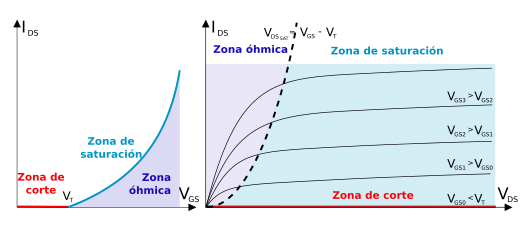
\includegraphics[width=0.6\textwidth]{./images/MOSFET_enhancement-mode_n-channel.svg.png}
                            \caption{Diagrama das regiões de operação do MOSFET.}

                        \end{figure}

                \end{itemize}

            Em circuitos digitais, os MOSFETs são usadas preferencialmente as regiões de corte e região ôhmica. Em circuitos analógicos é usado o transístor em modo de saturação, o que costuma fazer confusão com o modo de saturação dos transístores bipolares de junção que são substancialmente diferentes. A saturação nos MOS é análoga a Zona Ativa Direta dos TBJ.

        \subsection{Circuitos práticos}

            \begin{itemize}

                \item \textbf{AMPLIFICADOR DE BANDA LARGA:} O circuito mostrado na figura \ref{fig:amplificador} pode amplificar sinais que vão desde a faixa de áudio até 10 MHz\cite{newtoncbraga_mosfet_2025}.

                    \begin{figure}[htpb!]

                        \centering
                        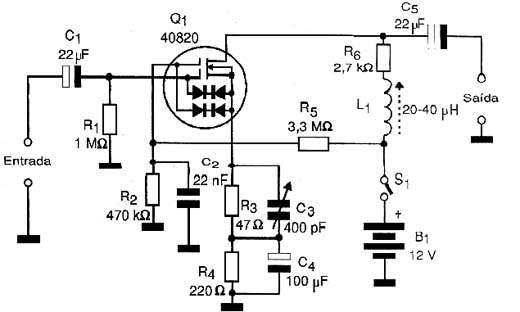
\includegraphics[width=0.6\textwidth]{./images/Amplificador banda larga.jpg}
                        \caption{Circuito do amplificador de banda larga.}
                        \label{fig:amplificador}

                    \end{figure}
                A faixa muito larga de frequências de operação e sua impedância de entrada da ordem de 1 M ? o torna ideal como etapa de entrada para instrumentos tais como frequencímetros ou mesmo osciloscópio.

                A intensidade máxima do sinal de entrada (a partir do qual temos a saturação) é da ordem de 100 mVrms.

                A amplitude máxima do sinal de saída é de 1 Vrms.

                O indutor que serve de carga para a saída é ajustado para se obter com o trimmer o ganho máximo do circuito na frequência de 10 MHz, mas dependendo da aplicação estes componentes podem ser alterados.

                Observe que uma das comportas tem uma polarização fixa dada por R2 e R3 de modo a levar o componente a uma corrente de repouso ideal para a aplicação.

                \item \textbf{SEGUIDOR DE FONTE}: Um seguidor de fonte é um amplificador que tem um ganho de tensão unitário, porém uma elevadíssima impedância de entrada e uma impedância muito baixa de saída. O circuito da figura \ref{fig:seguidor} mostra uma aplicação deste tipo que pode ser considerada equivalente ao seguidor de tensão normalmente feito com amplificadores operacionais.

                    \begin{figure}[htpb!]

                        \centering
                        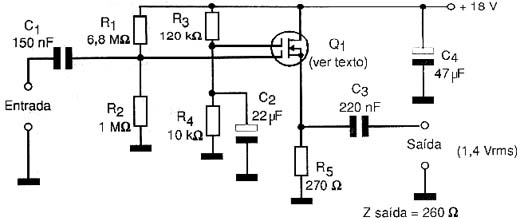
\includegraphics[width=0.6\textwidth]{./images/Seguidor de fonte.jpg}
                        \caption{Circuito do seguidor de fonte.}
                        \label{fig:seguidor}

                    \end{figure}

                Neste caso a amplitude máxima do sinal de entrada antes do qual se obtém a saturação é da ordem de 2 volts e a amplitude máxima do sinal de saída é da ordem de 1,5 Vrms.

                Dentre as aplicações recomendadas para este circuito podemos citar o casamento de impedância de fontes de sinais de áudio como, por exemplo, microfones.

                \item \textbf{PROVADOR DE BOBINAS E CAPACITORES}: O circuito da figura \ref{fig:provador} é uma ponte que serve tanto para medida de capacitâncias como indutâncias e faz uso de um transistor de efeito de campo MOS de canal duplo alimentado por uma tensão de 9 V.

                    \begin{figure}[htpb!]

                        \centering
                        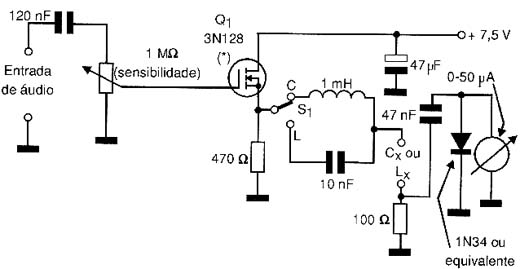
\includegraphics[width=0.6\textwidth]{./images/Provador de bobinas e capacitores.jpg}
                        \caption{Circuito do provador de bobinas e capacitores.}
                        \label{fig:provador}

                    \end{figure}

                O princípio de funcionamento é simples: aplica-se o sinal de um gerador de sinais na entrada, a frequência vai depender da ordem de grandeza da indutância ou da capacitância medida - normalmente ela estará entre 20 Hz e 20 kHz para medidas de capacitância entre 50 nF e 50 000 µF e indutâncias entre 5 mH e 6000 Hz com os valores de capacitância e indutância de referência usados.

                \item \textbf{ELETROSCÓPIO}: O circuito mostrado na figura \ref{fig:Eletroscópio} é de um simples eletroscópio eletrônico que pode ser usado com vantagem nas aulas de física substituindo o tradicional eletroscópio de folhas de ouro.

                    \begin{figure}[htpb!]

                        \centering
                        \includegraphics[width=0.6\textwidth]{./images/Eletroscópio.jpg}
                        \caption{Circuito do eletroscópio.}
                        \label{fig:Eletroscópio}

                    \end{figure}

                O circuito é alimentado por uma bateria de 9 V e o eletrodo sensor pode ser uma pequena argola de fio descascado ou ainda uma esfera de metal.

                Para testar atrite um pente ou caneta num pedaço de tecido e aproxime-o do sensor. A agulha do instrumento indicador deve oscilar fortemente.

            \end{itemize}

\section{Transistor Bipolar de Porta Isolada(IGBT)}

        O desenvolvimento do IGBT (do inglês, \textit{Insulated-Gate Bipolar Transistor}) foi motivado pela necessidade de um componente que unisse as melhores características de dois outros semicondutores: a alta impedância de entrada e a velocidade de comutação do MOSFET com a alta capacidade de corrente e baixa tensão de saturação do transistor bipolar (BJT).

        Os conceitos iniciais surgiram no final dos anos 1970. O engenheiro \textbf{B. Jayant Baliga}, enquanto trabalhava na General Electric, desenvolveu e demonstrou experimentalmente o primeiro dispositivo IGBT prático em 1982. A General Electric comercializou o primeiro dispositivo no mesmo ano.

        Um desafio crucial no início do desenvolvimento foi o fenômeno do \textit{"latch-up"} (travamento), uma condição onde a estrutura interna de tiristor do IGBT era ativada indevidamente, causando a perda de controle do dispositivo e sua eventual destruição. Esforços significativos foram feitos para suprimir essa trava. Em 1984, A. Nakagawa e sua equipe na Toshiba desenvolveram o conceito de design para IGBTs que não sofriam de \textit{latch-up}, o que permitiu a criação de componentes robustos e confiáveis. A Toshiba comercializou os primeiros produtos \textit{"non-latch-up"} em 1985, marcando o verdadeiro nascimento do IGBT moderno que conhecemos hoje \cite{wiki_igbt, onsemi_igbt}.


        \subsection{Tiristor}

        O tiristor diferente do IGBT,é um componente constituido de camadas que formam uma junção PNPN constituindo 4 camadas de formação tornando assim sua composição uma espécie de junção entre transistores do tipo PNP e NPN, seus terminais possuem ânodo,cátodo, e uma porta que funciona como um interrruptor, possuindo como modo de operação bloqueio reverso,direto e condução direta para controlar o fluxo de corrente no circuito. Suas aplicações são voltadas para sistemas de controle como controle de potência, motores e circuito de alarme.

        \begin{figure}[H]
            \centering
            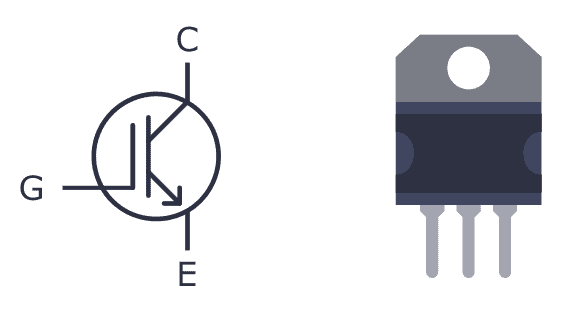
\includegraphics[width=0.45\textwidth]{./images/IGBT.png}
            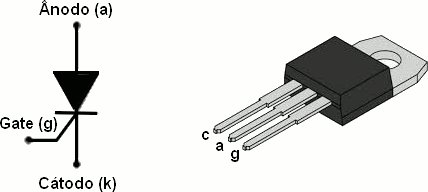
\includegraphics[width=0.45\textwidth]{./images/tiristor.png}
        \caption{À esquerda: IGBT. À direita: Tiristor.}
        \end{figure}


        \subsection{Estrutura do IGBT}

        O Transistor Bipolar de Porta Isolada (IGBT) possui uma estrutura vertical complexa, projetada para otimizar o bloqueio de altas tensões quando desligado e a condução de altas correntes com baixas perdas quando ligado. A sua construção é fundamentalmente uma evolução da tecnologia do MOSFET de potência vertical.

        \begin{figure}[!h]
            \centering
            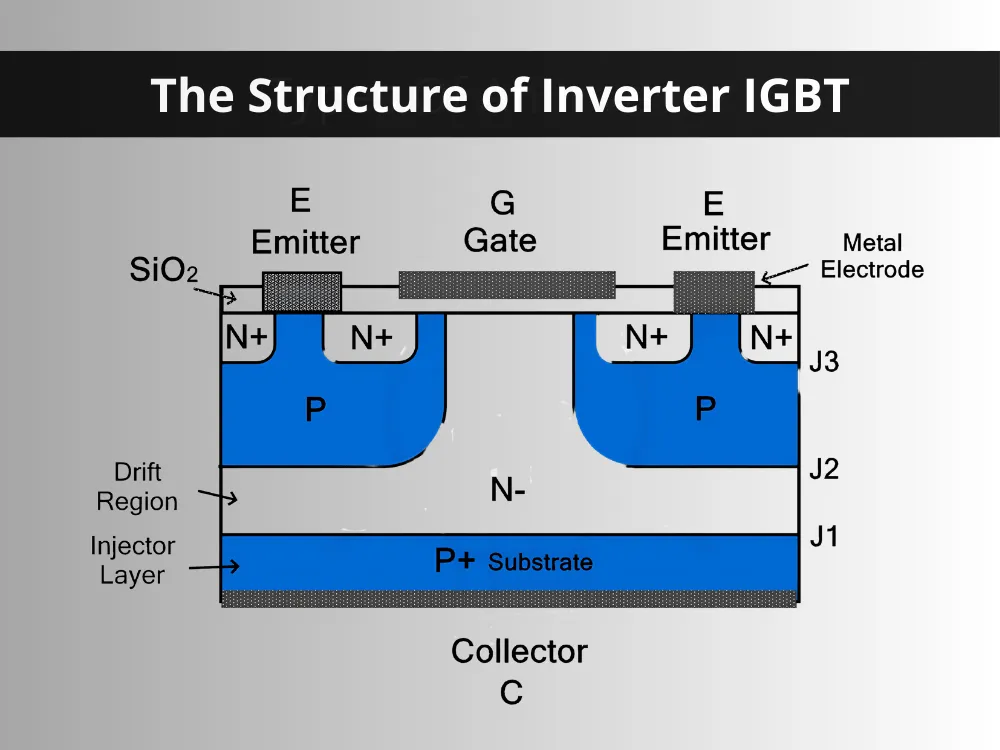
\includegraphics[width=0.6\linewidth]{images/The-structure-of-inverter-IGBT.png}
            \caption{Estrutura de um IGBT de canal N.}
            \label{fig:igbt_estrutura}
        \end{figure}

        \subsection{Construção Física}
        A estrutura de um IGBT de canal N é composta por quatro camadas semicondutoras alternadas, formando uma estrutura P-N-P-N, como mostrado na Figura \ref{fig:igbt_estrutura}. As camadas principais são:

        \begin{itemize}
            \item \textbf{Substrato P+ (Coletor):} Localizado na parte inferior do componente, atua como o terminal do Coletor. Esta camada é fortemente dopada e é responsável por injetar portadores minoritários (lacunas) na região de deriva durante a condução, um processo chave para a baixa tensão de saturação do IGBT.
            \item \textbf{Região de Deriva N- (Drift Region):} É uma camada espessa e levemente dopada. A sua espessura e dopagem determinam a capacidade de bloqueio de tensão do dispositivo. É nesta região que ocorre a \textbf{modulação de condutividade}, onde a injeção de lacunas pelo coletor aumenta drasticamente a condutividade, reduzindo a resistência e, consequentemente, a queda de tensão ($V_{CE(sat)}$).
            \item \textbf{Corpo P (Body):} Esta camada é onde o canal de condução é formado. O acionamento do gate atrai elétrons para a superfície desta camada, criando uma "ponte" (canal N) que conecta a região do emissor à região de deriva.
            \item \textbf{Regiões N+ (Emissor):} São regiões fortemente dopadas localizadas na superfície superior. O terminal de Emissor é metalizado em contato com estas regiões e com a região de corpo P.
            \item \textbf{Gate Isolado:} Assim como em um MOSFET, o terminal de Gate é feito de polissilício e é eletricamente isolado do corpo do semicondutor por uma fina camada de dióxido de silício ($\text{SiO}_2$).
        \end{itemize}

        \subsection{Estrutura Parasitária e Latch-up} A sequência de camadas P-N-P-N cria um Tiristor (ou SCR) parasitário, composto por um transistor PNP (formado pelas camadas P+, N-, P) e um transistor NPN (formado pelas camadas N-, P, N+). Se este tiristor for ativado, ele cria um caminho de baixa impedância entre o coletor e o emissor que não pode ser desativado pelo gate, um fenômeno destrutivo chamado \textbf{latch-up}. Designs modernos de IGBTs minimizam a probabilidade de \textit{latch-up} através de geometrias cuidadosas e dopagem otimizada para reduzir o ganho dos transistores parasitas.


        \begin{figure}[!h]
            \centering
            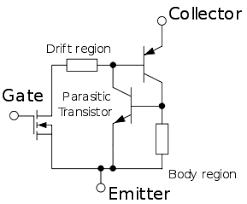
\includegraphics[width=0.6\linewidth]{images/igbt-circuit-diagram.png}
            \caption{Estrutura parasitária do tiristor em um IGBT.}
            \label{fig:igbt_latchup}
        \end{figure}

        \subsection{Tipos de Estrutura de Gate}
        Existem duas topologias principais para a estrutura do gate:
        \begin{itemize}
            \item \textbf{Gate Planar:} A estrutura mais antiga, onde o gate fica em uma superfície plana acima do corpo do componente.
            \item \textbf{Gate de Trincheira (Trench Gate):} Em designs mais modernos, o gate é construído em uma trincheira vertical. Esta abordagem aumenta a densidade de células no chip, resultando em menor resistência de condução ($R_{DS(on)}$) e melhor desempenho geral.
        \end{itemize}

        \begin{figure}[!h]
            \centering
            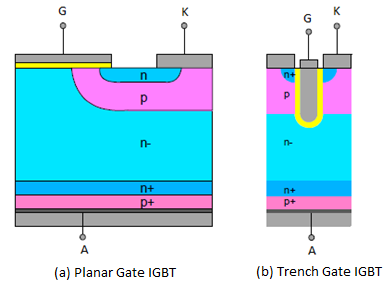
\includegraphics[width=0.6\linewidth]{images/planar_trench_gate.png}
            \caption{Comparação entre estruturas de gate planar e de trincheira.\cite{phdthesis}}
            \label{fig:igbt_gate_types}
        \end{figure}

        \subsection{Princípio de Funcionamento}
        O IGBT é um componente semicondutor de quatro camadas (PNPN) que combina uma estrutura de entrada MOS (\textit{Metal-Oxide-Semiconductor}) para controle e uma estrutura de saída bipolar para comutação de alta potência. Em sua estrutura equivalente, pode-se visualizar o IGBT como um MOSFET de canal N controlando um transistor PNP em uma configuração pseudo-Darlington, onde o coletor do IGBT é o emissor do PNP, e o emissor do IGBT é o coletor do PNP, passando pelo MOSFET de controle. Esta configuração única permite que o IGBT combine as melhores características de ambos os tipos de dispositivos: a alta impedância de entrada e facilidade de controle do MOSFET com a alta capacidade de condução de corrente e baixa queda de tensão do transistor bipolar. O resultado é um dispositivo que pode operar com altas tensões e correntes, mantendo perdas de condução relativamente baixas, características essenciais para aplicações de eletrônica de potência.

        \subsubsection{Acionamento} Para ligar o IGBT, uma tensão positiva é aplicada ao terminal de Gate (G) em relação ao Emissor (E), similar a um MOSFET. Essa tensão ($V_{GE}$) deve ser superior a uma tensão de limiar (\textit{threshold}), $V_{GE(th)}$. Ao ser aplicada, essa tensão cria um canal de condução (camada de inversão) na região P sob o gate, permitindo que elétrons fluam do emissor para a região de deriva N-. Essa injeção de elétrons na região N- causa uma injeção de lacunas da camada P+ (coletor), um fenômeno conhecido como \textbf{modulação de condutividade}. Essa modulação reduz drasticamente a resistência da região de deriva, permitindo que o IGBT conduza altas correntes com uma baixa queda de tensão ($V_{CE(sat)}$).

        \subsubsection{Corte} Para desligar o IGBT, a tensão no gate é removida ou negativada ($V_{GE} = 0V$ ou negativa). Isso desfaz o canal de condução, interrompendo o fluxo de elétrons. A corrente não cessa instantaneamente; há um pequeno tempo de atraso (\textit{turn-off delay time}) e um tempo de queda (\textit{fall time}), onde as portadoras minoritárias (lacunas) remanescentes na região de deriva se recombinam. Este processo gera a chamada \textit{"corrente de cauda"} (\textit{tail current}), uma característica distintiva do desligamento do IGBT.

        \subsection{Equações e Curvas Características}

        Embora a modelagem completa seja complexa, a operação do IGBT pode ser entendida por suas curvas características:

        \subsubsection{Curva de Transferência ($I_C$ vs $V_{GE}$)}
        Similar à de um MOSFET de potência, esta curva mostra que a corrente de coletor ($I_C$) só começa a fluir quando a tensão gate-emissor ($V_{GE}$) ultrapassa a tensão de limiar $V_{GE(th)}$. A partir daí, $I_C$ aumenta com $V_{GE}$. A relação pode ser aproximada pela equação:

        \[
        I_C = g_m \cdot (V_{GE} - V_{GE(th)})
        \]
        Onde $g_m$ é a transcondutância do dispositivo.

        \begin{figure}[!h]
            \centering
            
\includegraphics[width=0.6\linewidth]{images/curva_de_transferencia.png}
            \caption{Curva de transferência típica de um IGBT.}
            \label{fig:igbt_transfer}
        \end{figure}


        \subsubsection{\texorpdfstring{Curva de Saída ($I_C$ vs $V_{CE}$)}{Curva de Saída (IC vs VCE)}} Esta curva mostra a relação entre a corrente de coletor ($I_C$) e a tensão coletor-emissor ($V_{CE}$) para diferentes valores de $V_{GE}$.
        \begin{itemize}
            \item \textbf{Região de Corte:} Quando $V_{GE} < V_{GE(th)}$, o IGBT está desligado e apenas uma pequena corrente de fuga flui.
            \item \textbf{Região Ativa:} Onde $I_C$ é controlada por $V_{GE}$, e o IGBT opera como um amplificador (uso incomum).
            \item \textbf{Região de Saturação:} Quando o IGBT está totalmente ligado, $V_{CE}$ é muito baixa ($V_{CE(sat)}$) e o dispositivo se comporta como uma chave fechada. A $V_{CE(sat)}$ é a soma da queda de tensão em uma junção PN (diodo) e a queda de tensão no canal do MOSFET \cite{infineon_igbt_char}.
            \[
            V_{CE(sat)} \approx V_{J_{PN}} + V_{MOSFET}
            \]
        \end{itemize}

        \begin{figure}[!h]
            \centering
            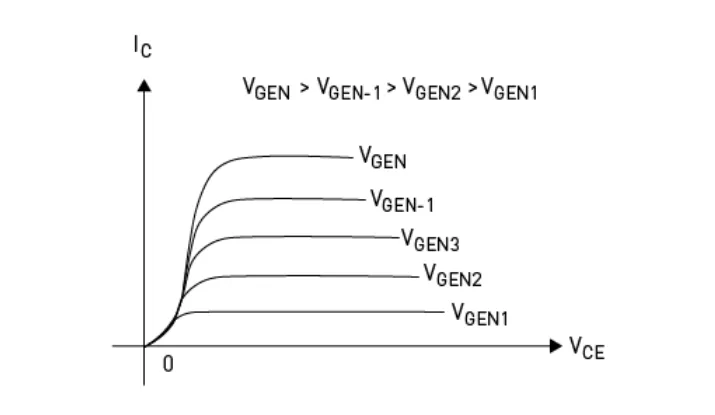
\includegraphics[width=0.6\linewidth]{images/curva_de_saida.png}
            \caption{Curva de saída típica de um IGBT.}
            \label{fig:igbt_output}
        \end{figure}

        \subsubsection{Regiões de Operação}
        O IGBT é projetado principalmente para operar como uma chave eletrônica, alternando entre dois estados principais:
        \begin{enumerate}
            \item \textbf{Modo de Corte (Forward Blocking Mode):} Ocorre quando $V_{GE} < V_{GE(th)}$. O dispositivo está desligado (chave aberta), bloqueando a passagem de corrente entre o coletor e o emissor, suportando altas tensões $V_{CE}$.
            \item \textbf{Modo de Condução (Conduction Mode):} Ocorre quando $V_{GE} > V_{GE(th)}$. O dispositivo está ligado (chave fechada), permitindo a passagem de alta corrente $I_C$ com uma baixa queda de tensão $V_{CE(sat)}$.
        \end{enumerate}
        Não possui uma capacidade de bloqueio reverso significativa, sendo inerentemente um dispositivo unidirecional \cite{mps_igbt}.

        \section*{Aplicações do IGBT}

        O IGBT é um componente de alta potência, ideal para aplicações de chaveamento em frequências de alguns kHz até dezenas de kHz, graças a esse fatores, ele é amplamente utilizado em diversas aplicações industriais e comerciais. A seguir, são descritas algumas das principais aplicações do IGBT:

        \begin{enumerate}
            \item \textbf{Inversor de Frequência Monofásico (Meia Ponte ou Ponte Completa):}
            \begin{itemize}
                \item \textbf{Propósito:} Converter uma tensão DC em uma tensão AC de frequência e amplitude variáveis. É a base para o controle de velocidade de motores AC (VFD - \textit{Variable Frequency Drive}).
                \item \textbf{Simulação:} Montar um circuito de meia ponte (\textit{half-bridge}) com dois IGBTs para gerar uma onda PWM. Utilizar uma carga indutiva-resistiva (RL) para simular um motor.
                \item \textbf{O que observar:} As formas de onda de tensão e corrente na carga, a "corrente de cauda" durante o desligamento e as perdas de comutação.
            \end{itemize}

            \item \textbf{Conversor Buck (Step-Down) de Alta Potência:}
            \begin{itemize}
                \item \textbf{Propósito:} Reduzir um nível de tensão DC para um nível mais baixo de forma eficiente. Usado em fontes de alimentação chaveadas de alta potência (SMPS).
                \item \textbf{Simulação:} Um circuito buck básico usa um IGBT como chave principal, um diodo rápido (\textit{freewheeling}), um indutor e um capacitor. O IGBT é acionado por um sinal PWM.
                \item \textbf{O que observar:} A regulação da tensão de saída ao variar o ciclo de trabalho (\textit{duty cycle}) e a eficiência do conversor.
            \end{itemize}

            \begin{figure}[htpb!]
                \centering
                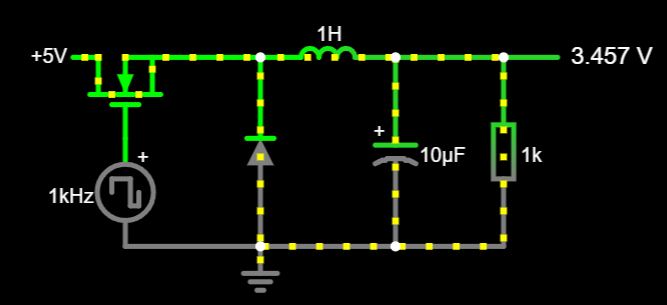
\includegraphics[width=0.5\textwidth]{./images/conversor_buck.png}
                \caption{Circuito de conversor buck com IGBT.}
            \end{figure}
            \begin{figure}[htpb!]
                \centering
                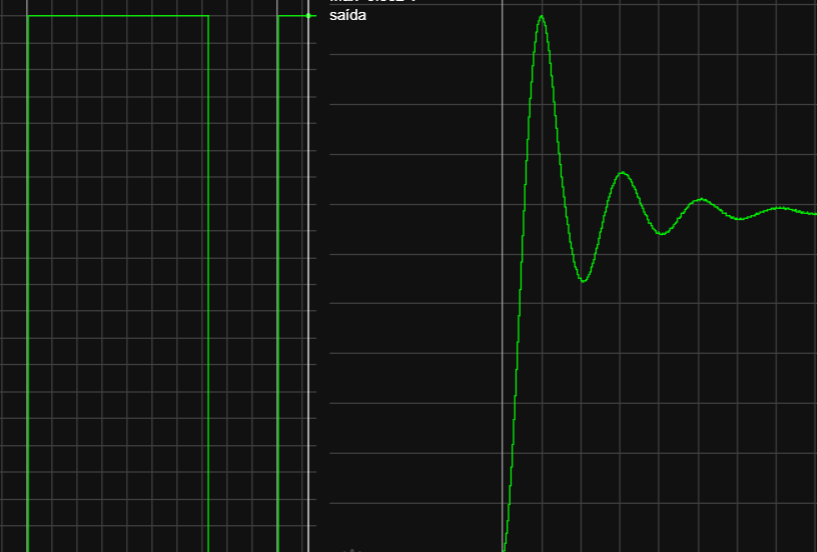
\includegraphics[width=0.5\textwidth]{./images/Entrada_saida.png}
                \caption{Exemplo de formas de onda de entrada e saída do conversor buck.}
            \end{figure}


            \item \textbf{Circuito de Controle de um Aquecedor por Indução:}
            \begin{itemize}
                \item \textbf{Propósito:} Gerar um campo magnético de alta frequência para aquecer objetos metálicos, como em fogões de indução.
                \item \textbf{Simulação:} Modelar um circuito ressonante RLC. O IGBT é usado em uma configuração de inversor para alimentar este circuito na sua frequência natural.
                \item \textbf{O que observar:} O chaveamento em tensão zero (ZVS) ou corrente zero (ZCS) para minimizar as perdas de comutação.
            \end{itemize}
        \end{enumerate}

\section{Conclusões}
    Este trabalho sintetiza as características fundamentais e as aplicações práticas dos três principais tipos de transistores de efeito de campo analisados: JFET, MOSFET e IGBT. A análise comparativa mostrou que cada tecnologia tem vantagens específicas que a tornam mais adequada a determinadas funções: o JFET destaca-se pela alta impedância de entrada e baixo ruído, sendo ideal para estágios de entrada de instrumentação e amplificadores de baixa potência; o MOSFET oferece alta impedância, comutação rápida e excelente desempenho em aplicações tanto digitais quanto analógicas de média potência; já o IGBT combina a facilidade de acionamento do MOSFET com a capacidade de conduzir altas correntes e suportar elevadas tensões, sendo a escolha natural para aplicações de potência (conversores, inversores e acionamento de motores).

    Além das diferenças elétricas, discutimos aspectos de projeto relevantes — como geometria do canal, dopagem, estrutura de gate e efeitos parasitários (por exemplo, o tiristor parasitário no IGBT que pode causar latch-up) — que influenciam diretamente parâmetros práticos: eficiência de condução, perdas de comutação, linearidade e comportamento térmico. Essas considerações reforçam que a seleção entre JFET, MOSFET e IGBT não é apenas uma questão de preferência, mas de adequação técnica ao requisito de circuito: sensibilidade ao ruído, faixa de frequência, dissipação de potência, e exigências de comutação.
    
    Em termos práticos, a conclusão principal é que entender as limitações físicas e os trade-offs de cada dispositivo permite projetar circuitos mais eficientes e confiáveis. Projetos de baixa potência e alta fidelidade favorecerão dispositivos de alta impedância e baixo ruído (como JFETs e MOSFETs de pequena sinal), enquanto aplicações de potência exigirão MOSFETs de potência ou IGBTs com topologias e técnicas de acionamento apropriadas para minimizar perdas e evitar fenômenos indesejáveis (como corrente de cauda e latch-up). Finalmente, a integração adequada de aspectos de projeto, simulação e testes experimentais é essencial para garantir desempenho e segurança em aplicações reais.

\newpage

\bibliography{referencia}

\end{document}
